\chapter{Расчет режимов спроектированной сети в ПВК RastrWin3}
\label{cha:растр_вин}

\section{Расчет режима наибольших нагрузок}

\textit{Отрегулированный режим НБ}

\begin{figure}[ht]
	\centering
	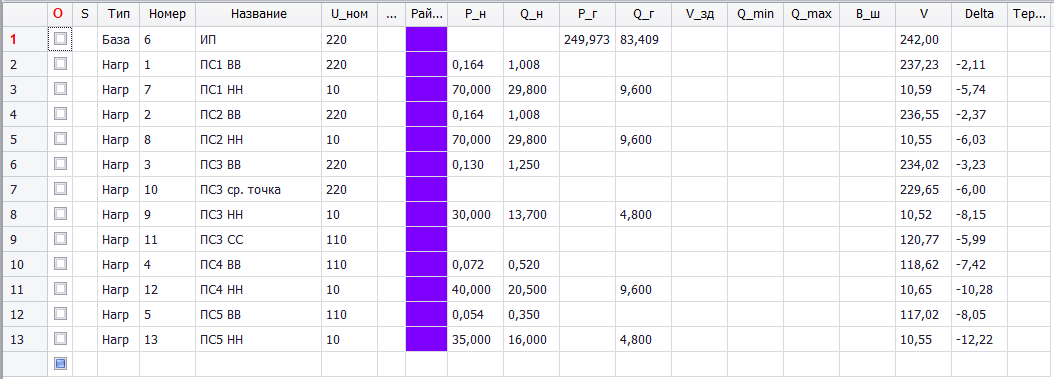
\includegraphics[width=1\textwidth]{inc/img/режим_нб_узлы_отрег}
	\caption{Параметры узлов в режиме НБ}
	\label{fig:узлы_нб}
\end{figure}

\begin{figure}[ht]
	\centering
	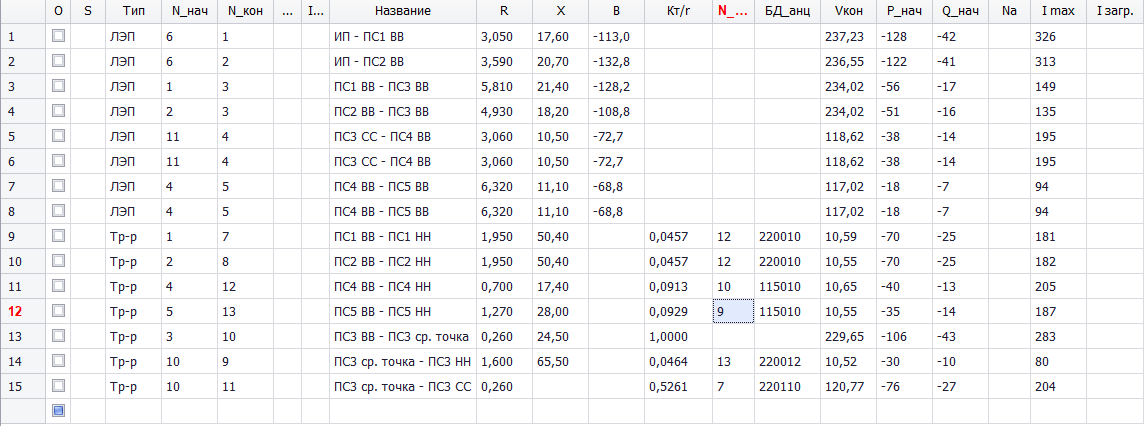
\includegraphics[width=1\textwidth]{inc/img/режим_нб_ветви_отрег}
	\caption{Параметры ветве в режиме НБ}
	\label{fig:ветви_нб}
\end{figure}

\begin{figure}[ht]
	\centering
	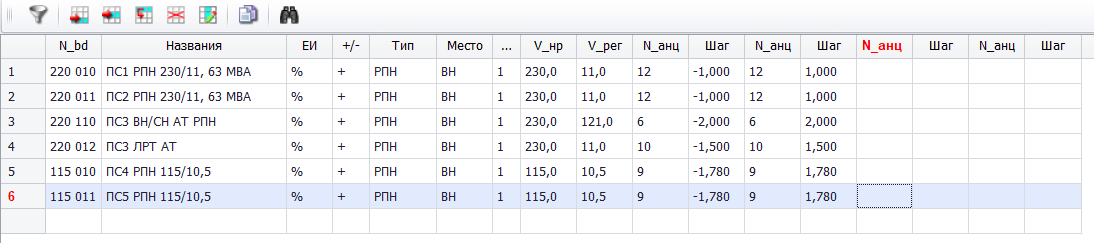
\includegraphics[width=1\textwidth]{inc/img/режим_нб_рпн}
	\caption{Параметры регулировочный устройств}
	\label{fig:анцапфы}
\end{figure}

\section{Расчет режима наименьший нагрузок (НМ)}

\begin{figure}[H]
	\centering
	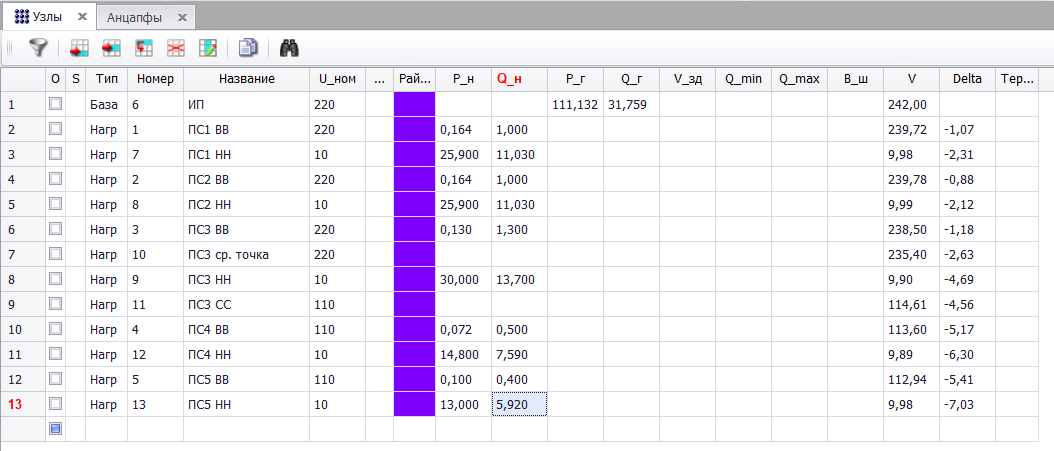
\includegraphics[width=1\textwidth]{inc/img/режим_нм_узлы_отрег}
	\caption{Параметры узлов в режиме НМ}
	\label{fig:узлы_нм}
\end{figure}

\begin{figure}[H]
	\centering
	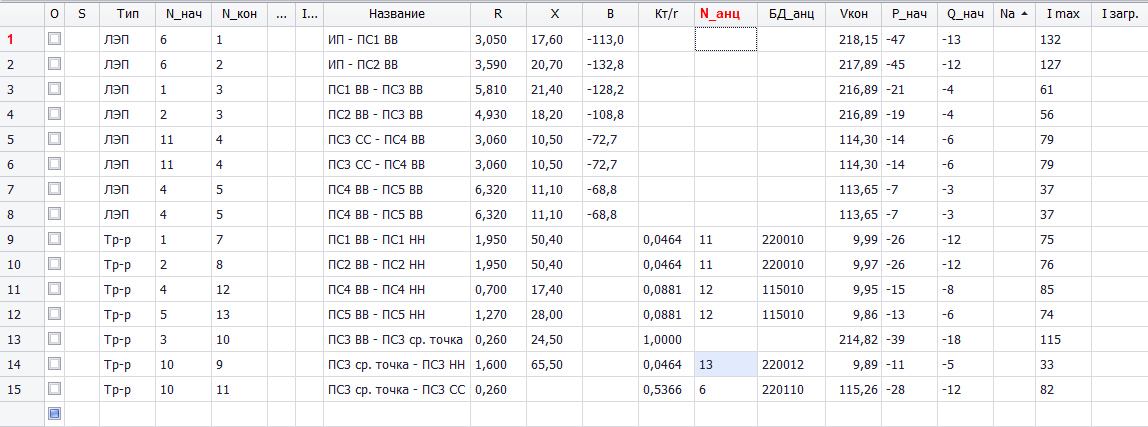
\includegraphics[width=0.8\textwidth]{inc/img/режим_нм_ветви_отрег}
	\caption{Параметры ветвей в режиме НМ}
	\label{fig:ветви_отрег}
\end{figure}

\section{Расчет послеаварийных режимов}

\textit{Отключение одной цепи наиболее загруженной линии К-1 в сети 220 кВ}

\begin{figure}[ht]
	\centering
	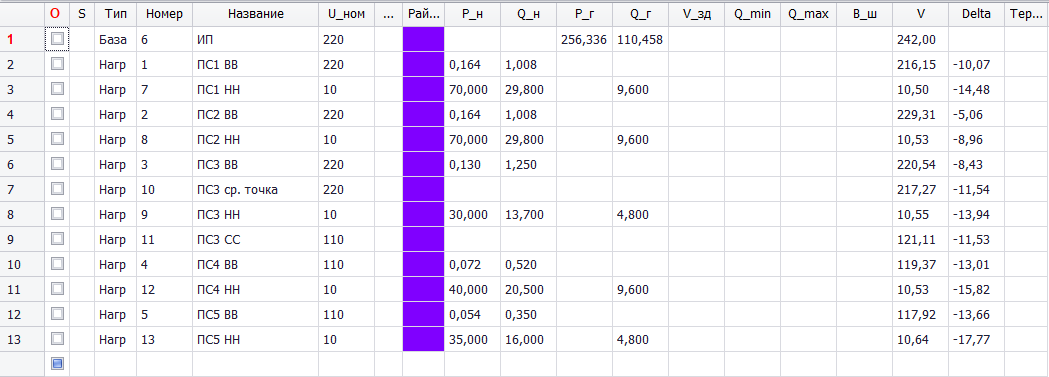
\includegraphics[width=1\textwidth]{inc/img/п_ав_220_кв_узлы_отрег}
	\caption{Параметры узлов в П/АВ режиме в сети 220 кВ}
	\label{fig:п/ав_в_сети_220_кв_узлы}
\end{figure}

\begin{figure}[ht]
	\centering
	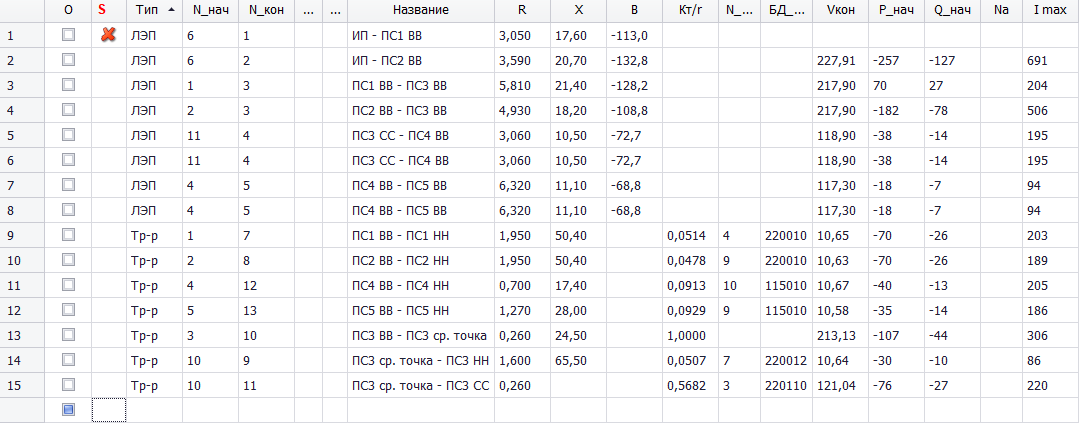
\includegraphics[width=1\textwidth]{inc/img/п_ав_220_кв_ветви_отрег}
	\caption{Параметры ветвей в П/АВ режиме в сети 220 кВ}
	\label{fig:п/ав_в_сети_220_кв_ветви}
\end{figure}

\textit{Отключение одной цепи наиболее загруженной линии 3-4 в сети 110 кВ}

\begin{figure}[ht]
	\centering
	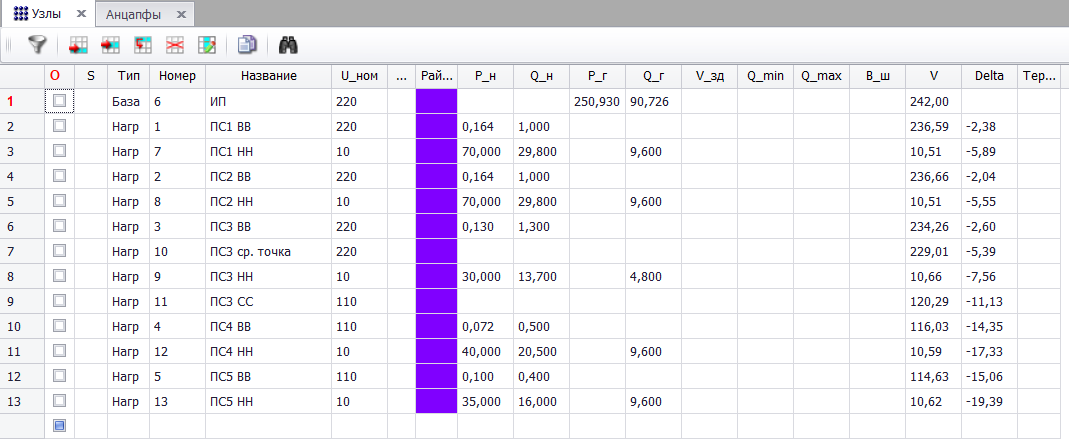
\includegraphics[width=1\textwidth]{inc/img/п_ав_110_кв}
	\caption{Параметры ветвей в П/АВ режиме в сети 220 кВ}
	\label{fig:п/ав_в_сети_110_кв_узлы}
\end{figure}

\begin{figure}[ht]
	\centering
	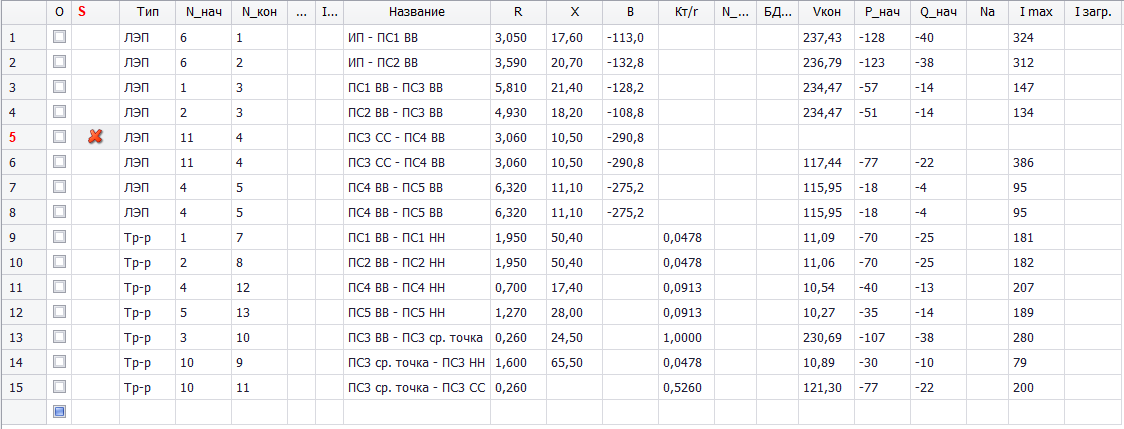
\includegraphics[width=1\textwidth]{inc/img/п_ав_110_кв_ветви}
	\caption{Параметры ветвей в П/АВ режиме в сети 110 кВ}
	\label{fig:п/ав_в_сети_110_кв_ветви}
\end{figure}